\documentclass[]{article}
\usepackage{amsmath}
\usepackage{amsfonts}
\usepackage{amssymb}
\usepackage{graphicx}
\usepackage[usenames, dvipsnames]{color}

%opening
\title{Parameter Sensitivity}
\author{Niall Mangan}

\begin{document}

\maketitle

\begin{abstract}

\end{abstract}
\section{Parameter Sensitivity}
\begin{figure}[h!]
	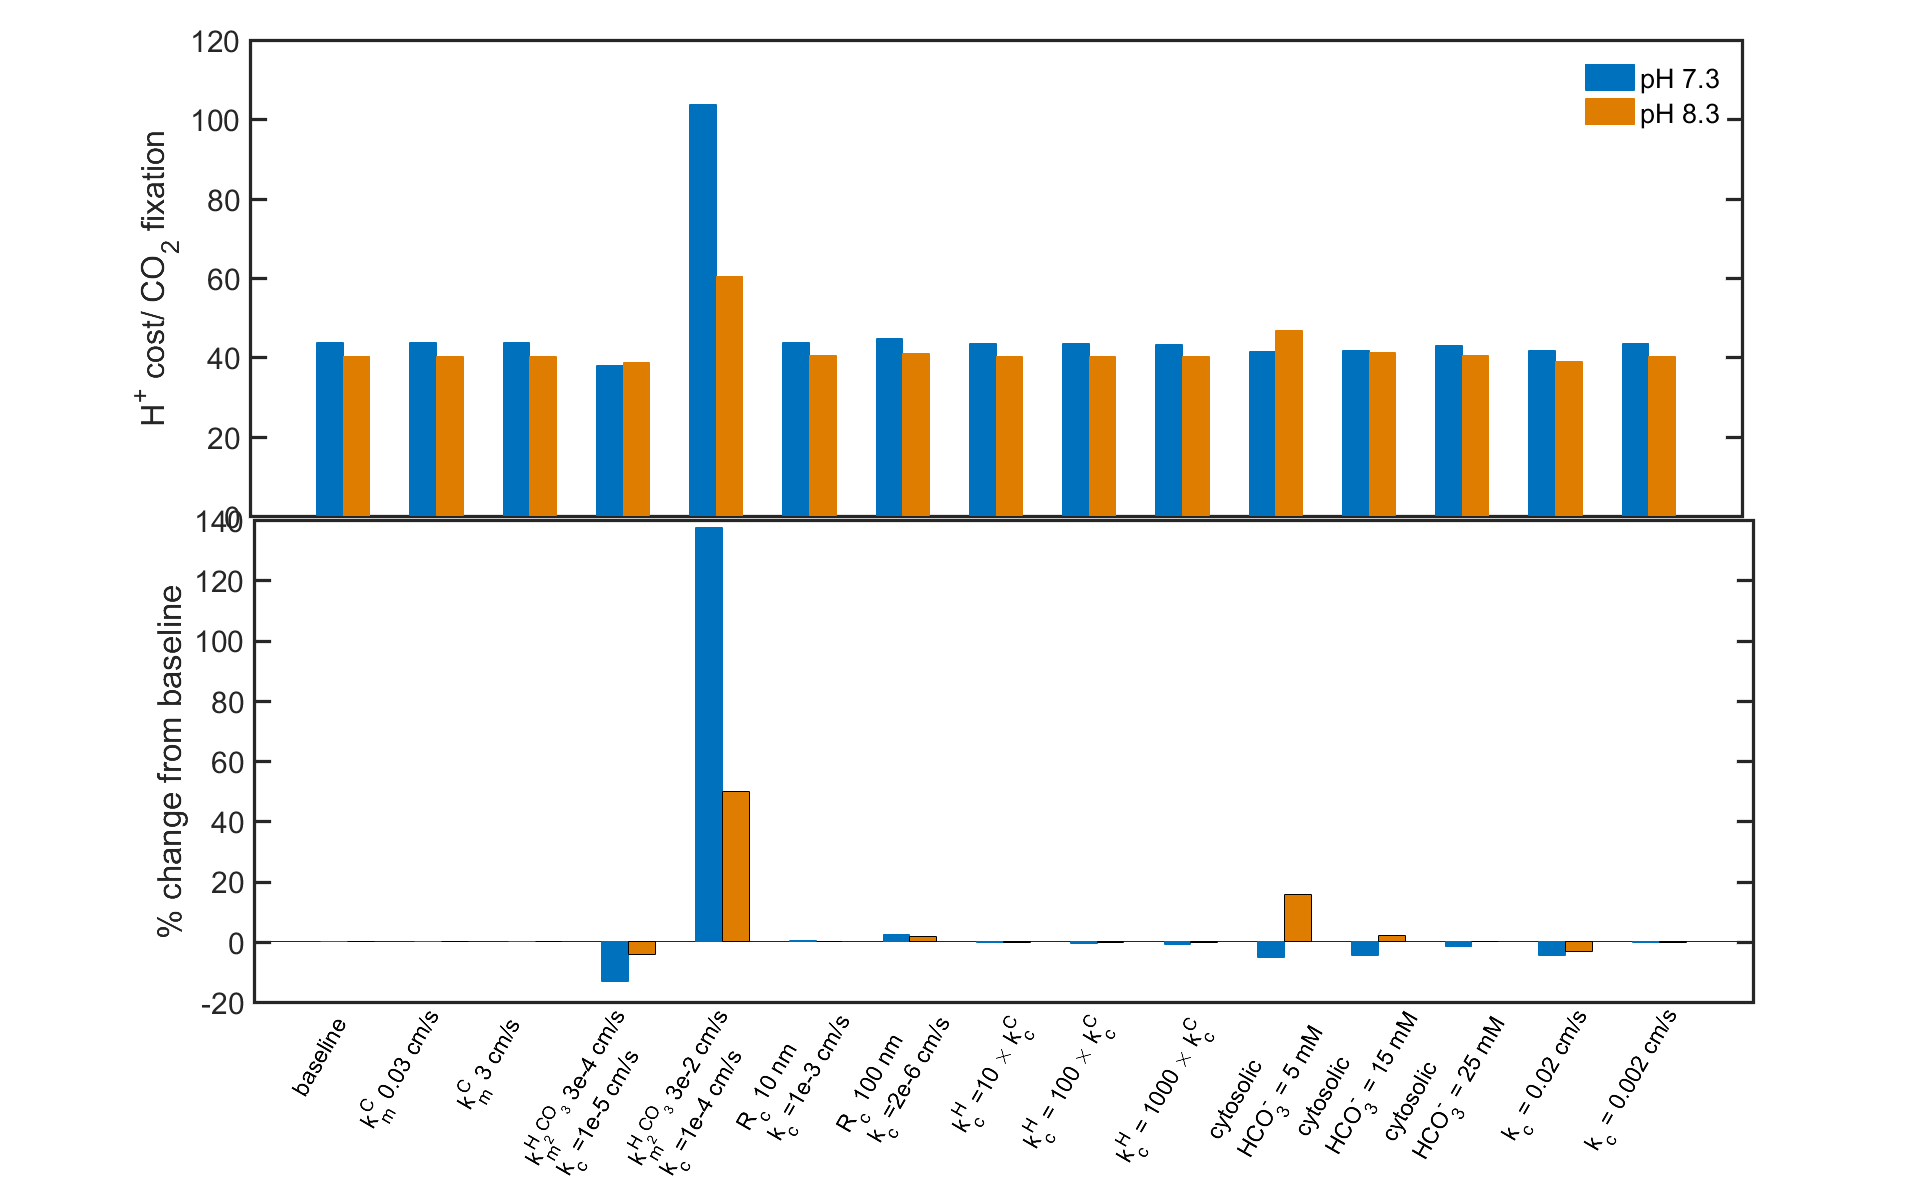
\includegraphics[width = \textwidth]{both.png}
	\caption{Cost and relative change from baseline for varying different parameters.For some parameters the carboxysome permeability is also changed to remain at optimal carboxysome permeability. Otherwise the main effect would be the shift away from optimum permeability.}
\end{figure}

\section{Equation when RuBisCO is saturated}
The analytic solution for the ${\rm CO_2}$ and ${\rm HCO_3^-}$ concentration in the carboxysome when RuBisCO is saturated is:

\begin{eqnarray}
C_{carboxysome} = \frac{N}{M} - \frac{R_c^3 V_{max}P}{3 M D}\\
H_{carboxysome} = K_{eq}(pH) C_{carboxysome}
\end{eqnarray}
where,

\begin{eqnarray}
N = (j_c+k_m^{eff}(pH_{out}))H_{out}((k_m^C+\alpha)G^C+\frac{D}{R_b^2}) + k_m^C C_{out} (k_m^{eff} G^H +\alpha G^C+\frac{D}{R_b^2}) \\
M = K_{eq}*k_m^{eff}\left((\alpha+ k_m^C)G^C +  \frac{D}{R_b^2}\right)
+ k_m^C\left(k_m^{eff} G^H + \frac{D}{R_b^2}\right) + \alpha k_m^{eff} G^H \\
P = ((\alpha + k_m^C)G^C+\frac{D}{R_b^2})(k_m^{eff} G^H + \frac{D}{R_b^2}) \\
G^C = \frac{D}{R_c^2 k_c^C} + \frac{1}{R_c}-\frac{1}{R_b} \\
G^H = \frac{D}{R_c^2 k_c^H} + \frac{1}{R_c}-\frac{1}{R_b} 
\end{eqnarray}
The derivation of this equation can be found in the supplementary material of (Mangan 2014). (\textcolor{red}{NOTE: In the derivation of the permeability equation in the SI it is clear that there are 2 additive terms - one for the interior pH and one for the exterior pH. It is not at all clear to me how those get integrated into the analytical equations. The code appears to do something a little different that what is written here. Let's discuss?}) Here we have made a few modifications: (1) kept track of the carboxysome permeability to ${\rm CO_2}$, $k_c^C$, and ${\rm HCO_3^-}$, $k_c^H$, independently, (2) substituted the pH dependent equilibrium constant for the carbonic anhydrase reaction, $K_{eq}(ph) = \frac{V_{ca} K_{ba}}{V_{ba}K_{ca}}$, (3) written the ${\rm CO_2} \rightarrow {\rm HCO_3^-}$ reaction with $\alpha$ as the linear reaction rate (in Mangan 2014 the linear rate was $\alpha/K_\alpha$), (4) we have replaced the membrane permeability to ${\rm HCO_3^-}$ with the effective membrane permeability to the bicarbonate pool, and designated when is dependent on the external pH. For all other $k_m^{eff}$ values it is dependent on the pH inside the cell.



\section{Reasonable reductions for physically relevant parameter values}
\subsection{Cell membrane permeabilty compared to diffusive velocities}
Examining equations (6) we note that for large carboxysome permeability $1/R_c$ will be the dominant term, and for smaller carboxysome permeability values the first term will be larger and dominate. Therefore $G^C \geq 1/R_c$. Studying the equations we note that the terms $((\alpha + k_m^C)G^C+\frac{D}{R_b^2})$ appears repeatedly. We use the following argument:
\begin{eqnarray}
(\alpha + k_m^C)G^C \geq (\alpha + k_m^C)/R_c>>D/R_b^2, \\
\; {\rm if} \; (\alpha +k_m^C)>> D R_c/R_b^2
\end{eqnarray}

For even a small 20 nm diameter ($R_c = 10^{-6}$ cm) carboxysome this will hold as $k_m^C \approx 0.3 $ cm/s and $D R_c/R_b^2 = 4 \times 10^{-3}$ cm/s from the values in Table S1. So the membrane permeability to ${\rm CO_2}$ could be an order of magnitude too high in our model and this would still be a reasonable assumption. Therefore we will substitute 
\begin{equation}
(\alpha + k_m^C)G^C + D/R_b^2 \approx (\alpha + k_m^C)G^C.
\end{equation}

Inserting this into equations (1-5) we get
\begin{multline}
C_{carboxysome} = \frac{(j_c+k_m^{eff}(pH_{out}))H_{out}(k_m^C+\alpha)G^C 
	+ k_m^C C_{out} (k_m^{eff} G^H +\alpha G^C+\frac{D}{R_b^2})}
{K_{eq} k_m^{eff}(\alpha+ k_m^C)G^C 
	 + k_m^C\left(k_m^{eff} G^H + \frac{D}{R_b^2}\right) + \alpha k_m^{eff} G^H} \\
-\frac{R_c^3 V_{max}(\alpha + k_m^C)G^C(k_m^{eff} G^H + \frac{D}{R_b^2})/(3D)}
{ K_{eq} k_m^{eff} \left(\alpha+ k_m^C \right)G^C 
	+ k_m^C\left(k_m^{eff} G^H + \frac{D}{R_b^2}\right) + \alpha k_m^{eff} G^H}.
\end{multline}
We can divide through by  $(k_m^C+\alpha)$ to obtain:
\begin{multline}
	C_{carboxysome} = \frac{(j_c+k_m^{eff}(pH_{out}))H_{out}G^C + \frac{k_m^C}{(k_m^C+\alpha)} C_{out} (k_m^{eff} G^H +\alpha G^C+\frac{D}{R_b^2})}
	{K_{eq} k_m^{eff} G^C  
		+\frac{k_m^C}{(k_m^C+\alpha)} \left(k_m^{eff} G^H + \frac{D}{R_b^2}\right) 
		+ \frac{\alpha}{(k_m^C+\alpha)}  k_m^{eff} G^H} \\
	-\frac{R_c^3 V_{max}G^C(k_m^{eff} G^H + \frac{D}{R_b^2})/(3D)}
	{ K_{eq} k_m^{eff} G^C + \frac{k_m^C}{(k_m^C+\alpha)}\left(k_m^{eff} G^H + \frac{D}{R_b^2}\right) 
		+ \frac{\alpha}{(k_m^C+\alpha)} k_m^{eff} G^H}.
\end{multline}

We now want to examine the remaining terms in the membrane permeability to ${\rm CO_2}$, $k_m^C$.

\subsection{Membrane permeability to ${\rm CO_2}$ has little effect.}
There are two parameter groupings in equation (12) containing $k_m^C$:
\begin{eqnarray}
\frac{k_m^C}{k_m^C + \alpha}\\
\frac{\alpha}{k_m^C + \alpha}
\end{eqnarray}

Therefore if $k_m^C > \alpha$ or ${\rm CO_2}\rightarrow {\rm HCO_3^-}$ conversion is negligible the first term (13) reduces to 1, and the second reduces to $1/k_m^C$. We will return to the case where this conversion is not negligible later. 

With these two simplifications we obtain: 
\begin{multline}
	C_{carboxysome} = \frac{(j_c+k_m^{eff}(pH_{out}))H_{out}G^C +  C_{out} (k_m^{eff} G^H +\alpha G^C+\frac{D}{R_b^2})}
	{K_{eq} k_m^{eff} G^C  
		+ \left(k_m^{eff} G^H + \frac{D}{R_b^2}\right) 
		+ \frac{1}{k_m^C}  k_m^{eff} G^H} \\
	-\frac{R_c^3 V_{max}G^C(k_m^{eff} G^H + \frac{D}{R_b^2})/(3D)}
	{ K_{eq} k_m^{eff} G^C + \left(k_m^{eff} G^H + \frac{D}{R_b^2}\right) 
		+ \frac{1}{k_m^C} k_m^{eff} G^H}.
\end{multline}

Examining equation (15), note that the only appearance of the membrane permeability to ${\rm CO_2}$ is now in the denominator which we can rewrite as $  k_m^{eff}(G^C K_{eq}+ \frac{G^H}{k_m^C})  + \left(k_m^{eff} G^H + \frac{D}{R_b^2}\right) $. Using this equation, we can write a strong bound on when the membrane permeability will effect the function of the CCM. 

We find $k_m^C$ has no significant effect when $K_{eq}G^C > \frac{G^H}{k_m^C}$ or $ k_m^C > \frac{G^H}{G^C K_{eq}}$. If we assume that the carboxysome permeability to ${\rm CO_2}$ will always be smaller than or equal to the permeability to ${\rm HCO_3^-}$ ($k_c^C\geq k_c^H$) then $G^H \geq G^C$ and $\frac{G^H}{G^C} \leq 1$, so $k_m^C$ will be negligible as long as $k_m^C > 1/K_{eq}$. For pH $> 6.6$, $1/K_{eq} > 0.3$ and therefore the assumed value of $k_m^C=0.3$ will be negligible. However, if the cell operated in a lower pH regime and the membrane permeability was substantially lower to $CO_2$ it would begin to effect the ${\rm CO_2}$ concentration. 

Thus far we have made a series of observations about the size of terms compared to the membrane permeability to ${\rm CO_2}$ and found that when $(\alpha +k_m^C)>> D R_c/R_b^2$, $k_m^C > \alpha$ and $ k_m^C > \frac{G^H}{G^C K_{eq}} \approx 1/K_{eq}$ the ${\rm CO_2}$ concentration in the carboxysome reduces to 
\begin{multline}
C_{carboxysome} = \frac{(j_c+k_m^{eff}(pH_{out}))H_{out}G^C +  C_{out} (k_m^{eff} G^H +\alpha G^C+\frac{D}{R_b^2})}
	{k_m^{eff}(G^C K_{eq} +  G^H) + \frac{D}{R_b^2} }\\
-\frac{R_c^3 V_{max}G^C(k_m^{eff} G^H + \frac{D}{R_b^2})/(3D)}
	{k_m^{eff}(G^C K_{eq} +  G^H) + \frac{D}{R_b^2} }.
\end{multline}

We can make a similar argument taking the equation for the ${\rm CO_2}$ concentration at the cell membrane:
\begin{multline}
C_{cytosol}(r = R_b) = \frac{k_m^C C_{out} - (\alpha + k_m^C)C_{carboxysome}}{(\alpha+k_m^C)G^C + D/R_b^2}G^C + C_{carboxysome}\\
\approx C_{out}
\end{multline}

This means that the ${\rm CO_2}$ leakage term will be negligible since the cytosolic ${\rm CO_2}$ concentration will be approximately equal to the external ${\rm CO_2}$ concentration. The ${\rm HCO_3^-}$ transport required to sustain a given internal inorgainc carbon pool will then be:

\begin{multline}
j_c H_{out} =  \left(\frac{R_c^3}{3 R_b^2}  V_{max}  -k_m^C \left( C_{out} - C_{cytosol} \right) - k_m^{eff} H_{out} + k_m^{eff} H_{cytosol} \right) \\ 
\; = \left(\frac{R_c^3}{3 R_b^2}  V_{max}  - k_m^{eff} H_{out} + k_m^{eff} H_{cytosol} \right)
\end{multline}

This equation is independent of the membrane permeability to ${\rm CO_2}$, as $H_{cytosol} = K_{eq}C_{cytosol}$ (\textcolor{red}{NOTE: NIALL this can't be true because then the cytosol would be in equilibrium. What did you mean here?}). This observation is consistent with the low flux of ${\rm CO_2}$ leakage in Figure 2.

\subsection{Without facilitated ${\rm CO_2}$ uptake external ${\rm CO_2}$ has little effect}

Unless conversion from ${\rm CO_2}$ to ${\rm HCO_3^-}$ is large we note that the second $C_{out}$ term in equation(15) is negligible for the regimes we study. We will revisit ${\rm CO_2}$ uptake and recycling later. Comparing this term against the first term in the numerator, again allows us to put a quantitative description on when this regime holds. Additionally we find that when the transport of ${\rm HCO_3^-}$ is significant ($j_c > k_m^{eff}(pH_{out})$) we arrive at

\begin{eqnarray}
	C_{carboxysome} = \frac{j_c H_{out}G^C - R_c^3 V_{max}G^C(k_m^{eff} G^H + \frac{D}{R_b^2})/(3D)}
	{k_m^{eff}(G^C K_{eq} +  G^H) + \frac{D}{R_b^2} }\\
	H_{carboxysome} = K_{eq} C_{carboxysome}
\end{eqnarray}




\section{Effect of Carboxysome permeability}


Recalling the equation for $G^C = \frac{D}{R_c^2 k_c^C} + \frac{1}{R_c}-\frac{1}{R_b}$, we can see that the carboxysome permeability to  ${\rm CO_2}$ will only matter if $ \frac{D}{R_c^2 k_c^C} >\frac{1}{R_c}$. In other words the carboxysome permeability to ${\rm CO_2}$, $k_c^C$, begins to effectively trap ${\rm CO_2}$ in the carboxysome when $k_c^C < \frac{D}{R_c} \approx 2$ cm/s for our base case of a 100 nm carboxysome ($R_c = 50$ nm). Similarly $G^H \approx \frac{D}{R_c^2 k_c^H}$ as $k_c^H \leq k_c^C < \frac{D}{R_c}$ (\textcolor{red}{NOTE: NIALL isn't $k_c^H \geq k_c^C$ in all the subsequent analyses? Seems like an error}). To begin let's examine the case when $k_c = k_c^C = k_c^H$.

In figure XX observe how the carboxysome radius shifts the onset of carboxysome permeability effecting the CCM function. (\textcolor{red}{NOTE: Odd that this is about size when the header is about permeability. As we discussed on the phone, radius variation is confusing. Let's consider dropping it or pushing it later in the SI?}) Both the highest carboxysome permeability where RuBisCO is saturated (blue lines) and carbonic remains unsaturated (maroon lines) and the optimal carboxysome permeability (that requiring the lowest ${\rm HCO_3^-}$ transport to achieve the same ${\rm CO_2}$ concentration) shift to lower permeability values with increasing carboxysome radii.

\begin{figure}
	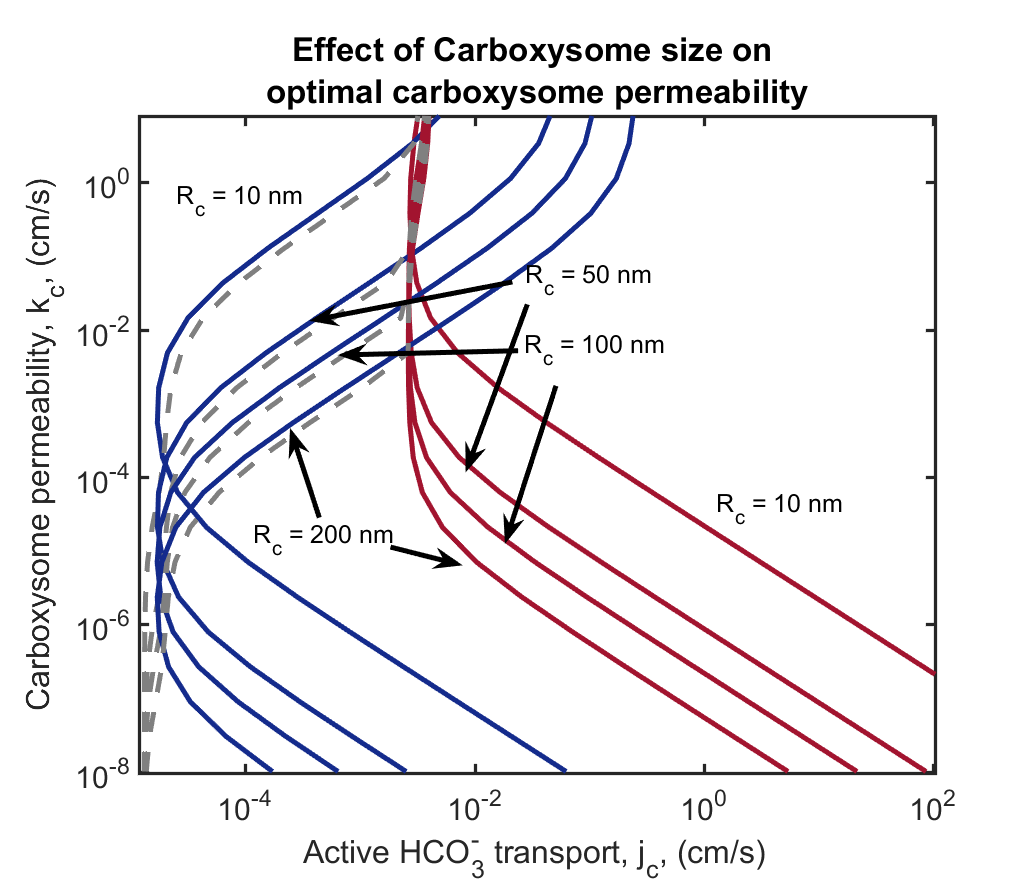
\includegraphics[width = \textwidth]{Rc_jcvskc.png}
	\caption{Changing the carboxysome radius shifts the onset of the carboxysome permeability effects and optimal carboxysome permeability. Blue lines show lines of constant concentration where  RuBisCO is saturated (saturated to the right), and maroon shows where carbonic anhydrase is saturated  (saturated to the right). Grey dashed lines shows where cytosolic ${\rm HCO_3^-}$ concentration is 30mM.}
\end{figure}
It is apparent that varying $R_c$ is simply shifting these lines vertically, if we plot $k_c \times R_c^2$ on the y-axis, as motivated by the term $\frac{D}{R_c^2 k_c^C}$. All the curves collapse! Therefore, the optimal carboxysome permeability or maximum carboxysome permeability must be considered in combination with $R_c$, if $R_c$ is varying. Until measurements of the carboxysome permeability are performed, if we want to consider smaller or larger carboxysomes we must also think about where we sit in the permeability phase space. Put another way, if you examine the cost of the CCM for varying $R_c$, it will be the same at the optimal $k_c$ value for each $R_c$ (and also the same for each maximal $k_c$ value supporting CCM function -- where maroon and blue lines meet).

\begin{figure}
	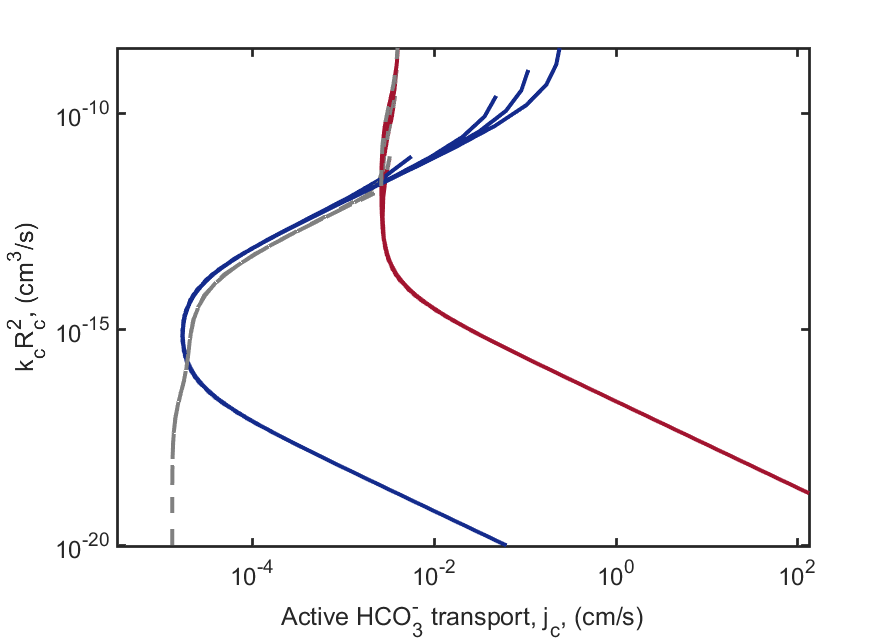
\includegraphics[width = \textwidth]{Rc_jcvskc_scaled.png}
	\caption{Same as previous figure, with y-axis scaled by $R_c^2$. All blue, maroon and grey dashed lines have collapsed.}
\end{figure}

\subsubsection{Different carboxysome peremability for ${\rm HCO_3^-}$}
An existing hypothesis in the CCM literature is that the carboxysome has differential permeability and is more permeable to ${\rm HCO_3^-}$ and less permeable to ${\rm CO_2}$. Intuitively this would allow more ${\rm HCO_3^-}$ into the carboxysome and trap more ${CO_2}$, thereby accumulating more inorganic carbon in the form of ${\rm CO_2}$. We use our model to test weather differential carboxysome permeability enables higher carboxysomal ${\rm CO_2}$ concentration for the same level of ${\rm HCO_3^-}$ transport. In the following figure we show the $k_c$ vs $j_c$ phase space where we have plotted the carboxysome permeability to ${\rm CO_2}$, $k_c^C$, on the y-axis. We plot different ratios (1, 10, 100, 1000) between $k_c^C$ and the carboxysome permeability to ${\rm HCO_3^-}$, $k_c^H = {\rm ratio} \times k_c^C$. 

\begin{figure}
	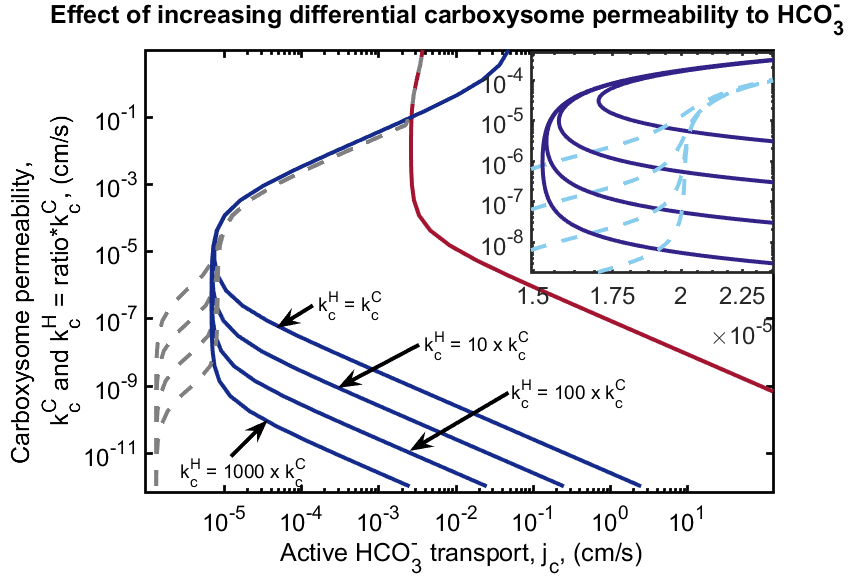
\includegraphics[width = \textwidth]{kcCkcHratio.png}
	\caption{Increasing the carboxysome permeability to ${\rm HCO_3^-}$ relative to ${\rm CO_2}$ mostly effects the required transport rates for ${\rm CO_2}$ carboxysome permeabilities below the optimum. Inset shows that there is a small decrease in necessary flux near the optimum.}
\end{figure}

Examining Figure XX, we see that making the carboxysome more permeable to ${\rm HCO_3^-}$ does not improve the function of the CCM as drastically as on might assume. The "turn on" of ${\rm CO_2}$ accumulation with decreasing permeability is unaffected by changes to $k_c^H$, and depends only on the permeability ${\rm CO_2}$, $k_c^C$.The "turn off" of accumulation for lower carboxysome permeabilities is greatly effected by the permeability of the carboxysome to ${\rm HCO_3^-}$, $k_c^H$. These two effects are exactly what we previously discussed as defining the carboxysome permeability optimum.

As we start at the top of the y-axis and decrease the carboxysome permeability the following occurs: At high permeability not enough ${\rm CO_2}$ is trapped, but ${\rm HCO_3^-}$ enters readily. As we moved to lower permeabilities ${\rm CO_2}$begins to be trapped, but there is a window where ${\rm HCO_3^-}$ still enters enough to supply the system. Eventually the carboxysome begins to restrict ${\rm HCO_3^-}$ entry. If the carboxysome is more permeable to ${\rm HCO_3^-}$ than to ${\rm CO_2}$ then the window where ${\rm CO_2}$ trapping is effective without restricting ${\rm HCO_3^-}$ entry broadens. The width of this window (on the y-axis) will also depend strongly on how much of the ${\rm CO_2}$ is being fixed.

The "turn off" of the optimum, caused by not allowing enough ${\rm HCO_3^-}$ into the carboxysome, does slightly increase the amount of transport required to saturate RuBisCO at the carboxysome optimum. The reduction in transport required, and therefore CCM cost is around 5\% when going from a $k_c^C$ to $k_c^H$ ratio of 1 to 1000.


%Not sure if we need analysis of the solution (also haven't checked this version carefully):
%\begin{equation}
%C_{carboxysome} = \frac{j_c H_{out}\frac{D}{R_c^2 k_c^C}- R_c^3 V_{max}\frac{D}{R_c^2 k_c^C}(k_m^{eff} \frac{D}{R_c^2 k_c^H}+ \frac{D}{R_b^2})/(3D)}
%{k_m^{eff}(\frac{D}{R_c^2 k_c^C} K_{eq} +  \frac{D}{R_c^2 k_c^H}) + \frac{D}{R_b^2} }
%\end{equation}
%
%dividing numerator and denominator through by $\frac{D}{R_c^2 k_c^C}$
%\begin{equation}
%C_{carboxysome} = \frac{j_c H_{out}- R_c^3 V_{max}(k_m^{eff} \frac{1}{R_c^2 k_c^H}+ \frac{1}{R_b^2})/3}
%{k_m^{eff}(K_{eq} +  \frac{k_c^C}{k_c^H}) + \frac{k_c^C R_c^2}{R_b^2} }
%\end{equation}

\section{Effect of membrane permeability to ${\rm H_2CO_3}$}

\begin{figure}[h!]
	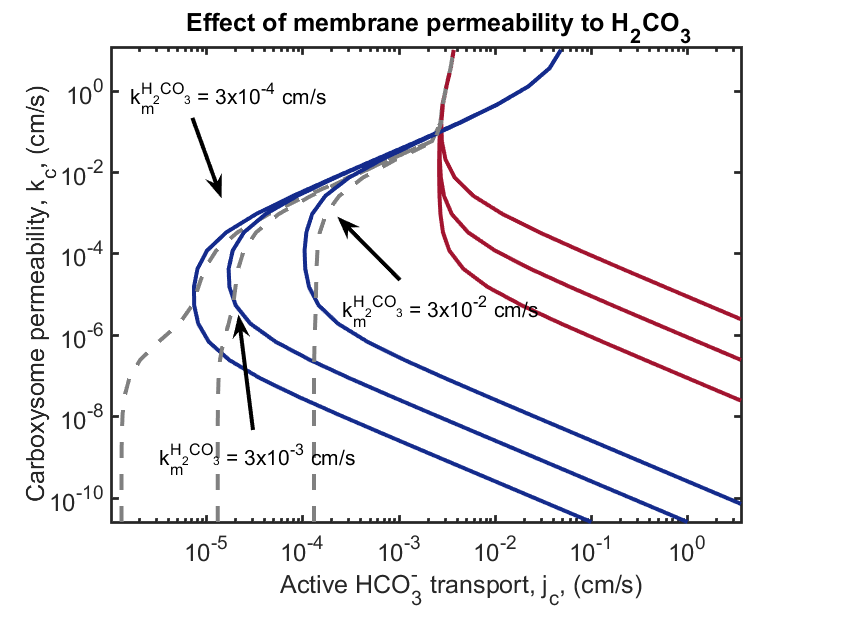
\includegraphics[width = \textwidth]{H2CO3permeability_jckc.png}
	\caption{CCM functionality space for varying membrane permeability to ${\rm H_2CO_3}$, $ k_m^{H_2CO_3}$. Blue lines indicate where RuBisCO is saturated. Red lines indicate where carbonic anhydrase is saturated. Grey dashed lines indicate where the ${\rm HCO_3^-}$ pool in the cytosol is 30mM. Each set of lines correspond to values  $ k_m^{H_2CO_3} = 3\times 10^{-4}, 3\times 10^{-3}, 3\times 10^{-2}$ from right to left.}
\end{figure}

The sensitivity of the cost to our assumption for the value of the membrane permeability to  ${\rm H_2CO_3}$ can be determined from the equation derived previously. If we are in a regime where ${\rm CO_2}$ leakage is negligible, as is the regime presented in the main paper, the second line holds. 
\begin{multline}
j_c H_{out} =  \left(\frac{R_c^3}{3 R_b^2}  V_{max}  -k_m^C \left( C_{out} - C_{cytosol} \right) -k_m^{eff}(pH_{out}) H_{out} +k_m^{eff}(pH_{in})  H_{cytosol} \right) \\ 
\; = \left(\frac{R_c^3}{3 R_b^2}  V_{max}  - k_m^{eff}(pH_{out}) H_{out} + k_m^{eff}(pH_{in}) H_{cytosol} \right)
\end{multline}
In this equation $k_m^{eff} = k_m^{H_2CO_3} \times 10^{(pK_1 - pH)}$. Therefore, the leakage of ${H_{total}}$ out of the cell will depend linearly on what we assume for $ k_m^{H_2CO_3}$. This linear dependence is past on to the active ${\rm HCO_3^-}$ transport required to replenish the leaked inorganic carbon, and therefore onto the CCM cost. In Figure XX you can see this effect, where going from $ k_m^{H_2CO_3} = 3\times10^{-2}$ to $ k_m^{H_2CO_3} = 3\times10^{-3}$ (an order of magnitude change), decreases the active ${\rm HCO_3^-}$ transport needed by an order of magnitude. Decreasing  to $ k_m^{H_2CO_3} = 3\times10^{-4}$ is a little less than an order of magnitude, indicating that the linear dependence breaks down and ${\rm CO_2}$ leakage would become important for that value. There is also an order of magnitude change in the optimal carboxysome permeability from ${\rm 10^{-4}}$ to ${\rm 10^{-5}}$ across the 2 order of magnitude change in $ k_m^{H_2CO_3}$ we are checking.



\section{Selection and effect of cytosolic ${\rm HCO_3^-}$ pool size}

\begin{figure}[h!]
	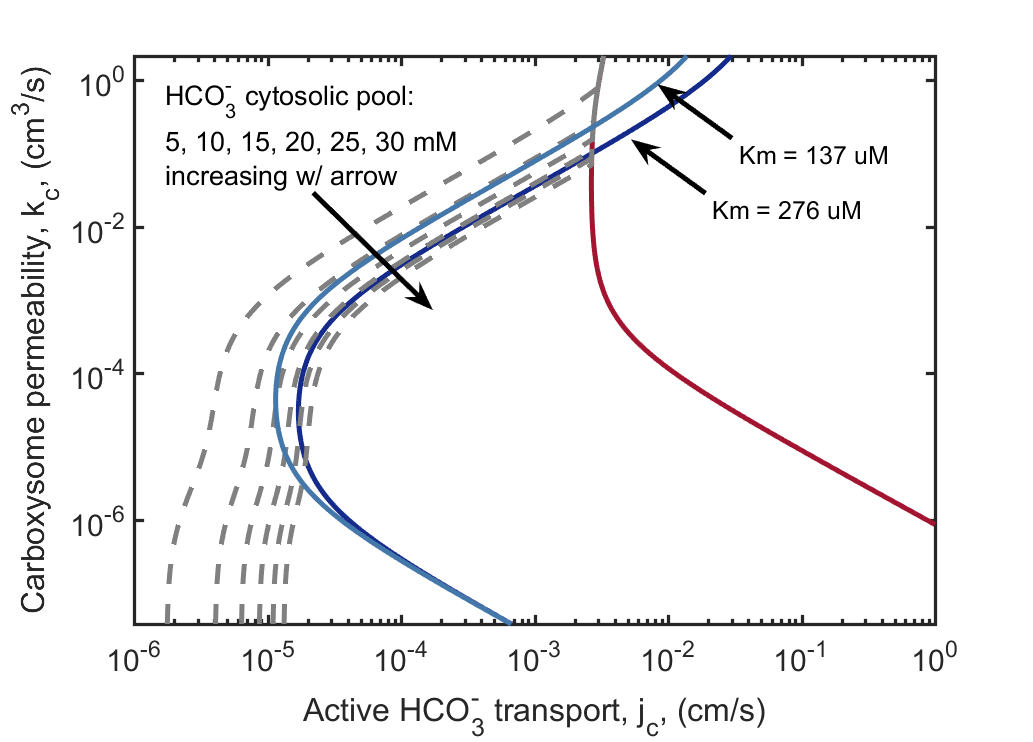
\includegraphics[width = \textwidth]{HcytoPool.png}
	\caption{CCM functionality space showing carboxysome permeability and ${\rm HCO_3^-}$ transport rates resulting in varying cytosolic ${\rm HCO_3^-}$ pool. Grey dashed lines indicate where the ${\rm HCO_3^-}$ pool in the cytosol is 5, 10, 15, 20, 25, and 30 mM. Blue lines indicate where RuBisCO is saturated. Red lines indicate where carbonic anhydrase is saturated.  }
\end{figure}

The ${\rm HCO_3^-}$ cytosolic pool we assume in our cost calculation has a large effect on the absolute values for the cost calculation. The dependence of ${\rm HCO_3^-}$ transport required to support a given internal cytosolic pool can also be seen in the equation in the previous section.  

In Figure XX the active ${\rm HCO_3^-}$ transport and carboxysome permeability values required to achieve a particular cytosolic pool are shown. For the RuBisCO half-max values assumed in the main text $K_m = 276 \; \mu M$ at internal pH 8, internal ${\rm HCO_3^-}$ cytosolic pools between 20 and 50 mM are required to saturated RuBisCO. For lower $K_m$ values, lower cytosolic pools would be required.
Additionally, as the $K_m$ values are pH dependent, the internal pH of the cell will effect when saturation takes place.

It has recently been suggested that cytosolic ${HCO_3^-}$ pools of around 5-10 mM can saturate RuBisCO. As was discussed in Whitehead et al., this is only possible with our given understanding of the CCM mechanism if the pH in the carboxysome is lower than the rest of the cell, or if the carbonic anhydrase does not act to bring ${\rm CO_2}$ and ${\rm HCO_3^-}$ into equilibrium. Either of these possibilities seems physically questionable given out current understanding of the diffusion rate of protons and the mechanism of carbonic anhydrase -- its speed is considered linked to its lack of directionality.
\section{When can ${\rm CO_2}$ scavenging have an effect}

Next we examine for which parameter regimes ${\rm CO_2} \rightarrow {\rm HCO_3^-}$ conversion activity acts as facilitated uptake, resulting in a flux of ${\rm CO_2}$ into the cell, or scavenging, reducing the leakage of ${\rm CO_2}$ out of the cell. As written, the conversion activity does not discriminate between ${\rm CO_2}$ that has recently diffused into the cell and ${\rm CO_2}$ which has already been in the carboxysome, but leaked back out. In other words, we do not "trace" the history of each ${\rm CO_2}$ molecule, or even model each ${\rm CO_2}$ molecule explicitly as we treat concentrations. Therefore, we must think about the net ${\rm CO_2}$ flux at the cell membrane. 

When there is a net flux of ${\rm CO_2}$ out of the cell, there is by definition, no facilitated uptake. If there is zero net flux of ${\rm CO_2}$ at the cell membrane, then the cell is scavenging 100\% of the ${\rm CO_2}$ leaking out of the carboxysome. If there is net flux of ${\rm CO_2}$ into the cell, then not only is the conversion mechanism scavenging all ${\rm CO_2}$ leaking out of the cell, but also reducing the cytosolic ${\rm CO_2}$ concentration below the external concentration and facilitating uptake.

\begin{figure}[h!]
	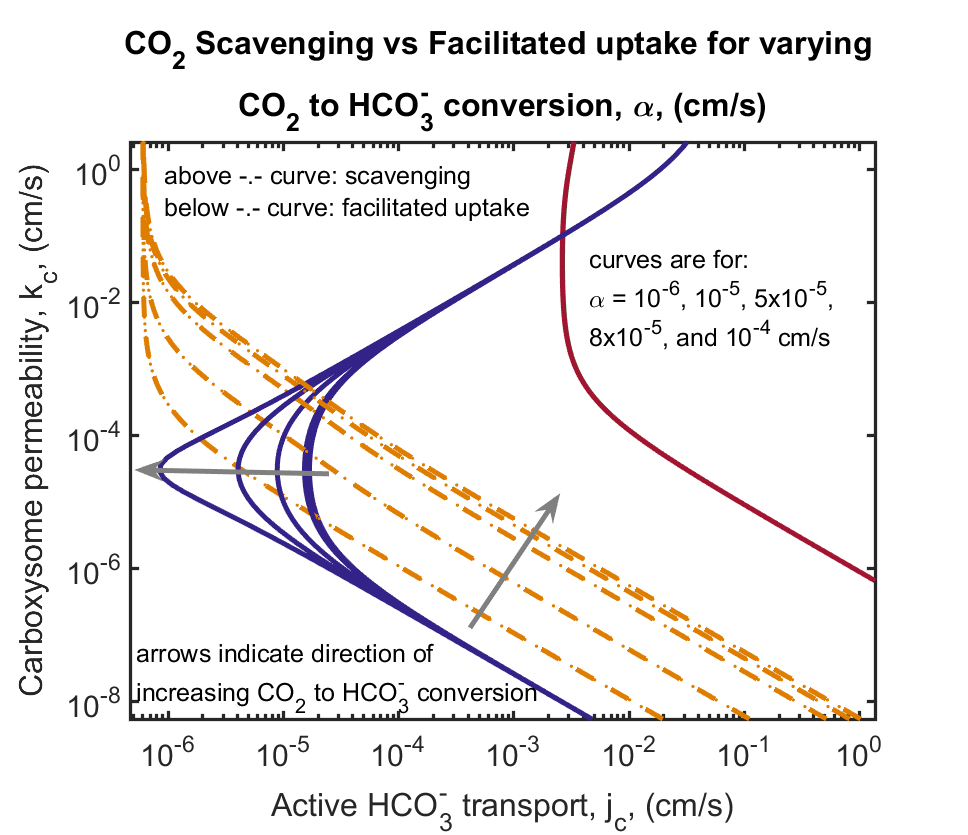
\includegraphics[width = \textwidth]{alpha_scavenging.png}
	\caption{Effect of ${\rm CO_2} \rightarrow {\rm HCO_3^-}$ conversion on the active transport vs carboxysome permeability plot. RuBisCO is unsaturated to the left of the blue line and saturated to the right. Carbonic anhydrase is unsaturated to the left of the red line and saturated to the right. Orange dashed lines show where the ${\rm CO_2}$ flux across the membrane is zero. Above/to the right of an orange dashed line there is net ${\rm CO_2}$ leaking out of the cell, and the main function of the conversion is scavenging. Below and to the left of an orange line the net ${\rm CO_2}$ flux at the cell membrane is into the cell, and conversion is both scavenging and facilitating ${\rm CO_2}$ uptake. Multiple lines are for increasing  ${\rm CO_2} \rightarrow {\rm HCO_3^-}$ conversion strength in the direction of the grey arrows. }
\end{figure}

From Figure XX it is evident that increasing ${\rm CO_2} \rightarrow{\rm HCO_3^-}$ decreases the need for active  ${\rm HCO_3^-}$ uptake at optimal carboxysome permeability. We can also determine when the conversion mechanism switches from being primarily a scavenging mechanism to also acting as facilitated uptake. The orange dashed lines show the active ${\rm HCO_3^-}$ transport rate for each carboxysome permeability $k_c$ value where the net ${\rm CO_2}$ flux at the cell membrane is zero. Above this line the system is scavenging and below it the system is scavenging and causing facilitated uptake. We have plotted these curves for increasing ${\rm CO_2} \rightarrow{\rm HCO_3^-}$ conversion strengths. 

For $\alpha = 10^{-6}$ cm/s, the system is not facilitating uptake of ${\rm CO_2}$ for the optimal permeability. At this point the minimum active ${\rm HCO_3^-}$ transport rate required to saturate RuBiSCO is approximately the same as without the ${\rm CO_2}$ conversion mechanism. For higher ${\alpha}$ the conversion system is scavenging at the optimal carboxysome permeability. In this case the system requires less ${\rm HCO_3^-}$ transport because ${\rm CO_2}$ conversion is acting as facilitated uptake, and contributing to the internal inorganic carbon pool. Note that the absolute flux from scavenging and facilitated uptake will vary drastically over this space. 

In the main text we showed that the loss of ${\rm CO_2}$ from leakage out of the cell is about an order of magnitude smaller than ${\rm HCO_3^-}$ leakage without ${\rm CO_2}$ conversion. When we are at optimal carboxysome permeability, scavenging will have little effect, because there is just not very much ${\rm CO_2}$ in the cytosol to scavenge. At higher carboxysome permeabilities though, the scavenging mechanism could compensate and matter much more. Thus the relative importance of the ${\rm CO_2}$ conversion mechanism for scavenging vs facilitated uptake depends highly on the yet experimentally undetermined carboxysome permeability.

%We can define the \% of ${\rm CO_2}$ scavanged compared to that leaked out of the carboxysome as:
%\begin{equation}
%S_\% = \frac{k_c(C_{carboxysome} - C_{cytosol}(R_c))}{k_m^C(C_{cytosol}(R_b)-C_{out})}
%\end{equation}
%Our analytically derived function for the cytosolic ${\rm CO_2}$ concentration as a function of the radius:
%\begin{equation}
%C_{cytosol} = \frac{k_m^C C_{out} - (\alpha-k_m^C) C_{carboxysome}}{(\alpha+k_m^C)G^C +\frac{D}{R_b^2}}\left(\frac{D}{k_c^C R_c^2} + \frac{1}{R_c} - \frac{1}{r}\right) +C_{carboxysome}
%\end{equation}
%We can use equation (24) in equation (23) and rearrange equation (23) to find the concentration of ${\rm CO_2}$ in the carboxysome resulting in a particular scavenging percentage. This can then be plotted on the ${\rm HCO_3^-}$ transport vs carboxysome permeability plot to see where the functionality is important.
%\begin{equation}
%C_{carboxysome}(S_\%) = \frac{(k_m^C S_\% ((\alpha + k_m^C)G^C + \frac{D}{R_b^2})- k_m^C(k_m^C S_\% G^C +\frac{D}{R_c^2}))C_{out}}{k_m^C S_\% ((\alpha + k_m^C)G^C + \frac{D}{R_b^2})- (\alpha+k_m^C)(k_m^C S_\% G^C +\frac{D}{R_c^2})}
%\end{equation}

To identify when facilitated uptake starts, we can find for what ${\rm CO_2}$ concentration in the carboxysome the flux at the cell membrane is zero, or when  $C_{cytosol}= C_{out}$. 
\begin{equation}
{\rm CO_2 \; flux} = k_m^C(C_{cytosol}(R_b)-C_{out}).
\end{equation}

We do not know enough about the ${\rm CO_2 \rightarrow HCO_3^-}$ mechanism to estimate a cost in the way we have done for ${\rm HCO_3^-}$ uptake. Therefore we cannot asses the effect of conversion on the cost.

%\begin{equation}
%C_{csome}(C_{cytosol}(R_b)= C_{out}) = C_{out} (1+(\alpha + k_m^C)G^C \frac{R_b^2}{D} - \frac{k_m^C R_b^2}{D})
%\end{equation}




\end{document}